\chapter{Muistinhallinta} \label{Toinen luku}

Ohjelman muistin rakenteen ymmärtäminen on erityisen tärkeää tehokkaan muistin käytön saavuttamiseksi. Seuraavissa luvuissa tullaan esittelemään miten muistin allokointi ohjelmissa toimii
ja millaisista muistialueista ohjelman muisti koostuu. Huomioitavaa on, että seuraavaksi esiteltävä muistirakenne on tyypillisin muistirakenne, mistä tietokoneohjelman muisti koostuu. Ohjelman muistin rakenteeseen vaikuttaa mm. käytössä oleva suoritinarkkitehtuuri, ohjelmointikielen kääntäjä sekä kääntäjien tarjoamat muistin optimointityökalut.

\section{Ohjelman muisti}

Ohjelman muisti jakautuu erilaisiin muistialueisin. Koodisegmentti sisältää varsinaisesti ajettavan ohjelman binäärin eli ohjelmatiedoston, jonka prosessori suorittaa. Lisäksi ohjelmalla on olemassa datasegmentti, joka koostuu alustetusta datasta ja alustamattomasta datasta. Alustetun datan alueeseen kuuluvat globaalit ja staattiset muuttujat sekä vakioarvoiset muuttujat, joille on alustettu jokin arvo. Alustamattomassa data-alueessa on kaikki alustamaton data eli muuttujat, jotka ovat esitelty (declare), mutta joille ei ole annettu mitään arvoa.\cite{mmic2010} Näiden muistialueiden data allokoidaan ajettavan ohjelman muistiin jo käännön aikana (compile time) eli ohjelmointikielen kääntäjän kääntäessä lähdekoodin. Ohjelmalla on lisäksi kaksi muistialuetta pino ja keko, joiden data allokoidaan vasta ajoaikana (runtime) eli kun ohjelman itse suorittaminen aloitetaan.

\begin{figure}[tbh]
{\begin{centering}
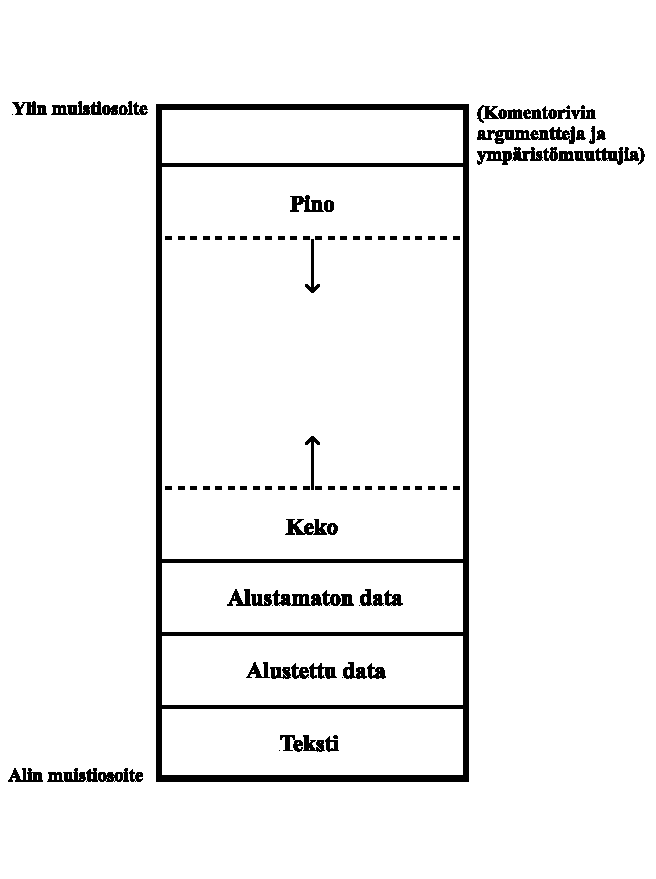
\includegraphics[width=0.6\textwidth]{kuvat/muistin_rakenne.pdf}
\par\end{centering}}
\caption{Ohjelman muistin rakenne\cite{mmic2010} (suomennettu kuva lähteestä)}
\end{figure}

/**Koodin pätkä**/

\subsection{Pino}
\subsection{Keko}

\section{Muistin allokointi ohjelmointikielissä}

Muistia voidaan allokoida ohjelmalla kahdella tavalla, staattisesti tai dynaamisesti.